%
% beispiele.tex
%
% (c) 2020 Prof Dr Andreas Müller, Hochschule Rapperswil
%
\subsection{Beispiele
\label{subsection:qam:beispiele}}
Die Quadratur-Amplituden-Modulation ermöglicht, im Vergleich zur
Trägerfrequenz langsam veränderliche zweidimensionale Signale zu
übertragen und wieder zu rekonstruieren.
Der besondere Nutzen dieser Technik ist jedoch, dass sie viele
ältere Modulationsverfahren als Spezialfälle enthält, wie in
diesem Abschnitt gezeigt werden soll.

\subsubsection{Amplitudenmodulation}
{\em Amplitudenmodulation} konnten wir verstehen, bevor wir $Q(t)$ kannten,
sie ist der Spezialfall $Q(t)=0$.
Für ein Audiosignal $A(t)$ mit $A(t)<1$ wird $I(t)=1+A(t)$ verwendet.
Das in Europa weitgehend bereits durch Digitalradio ersetzte 
Mittelwellenradio (AM) verwendet Amplitudenmodulation.
Bis 2025 werden in Europa alle Radiostationen digitalisiert, damit
wird AM für den Rundfunk aussterben.

\subsubsection{Phasenmodulation}
\begin{figure}
\centering
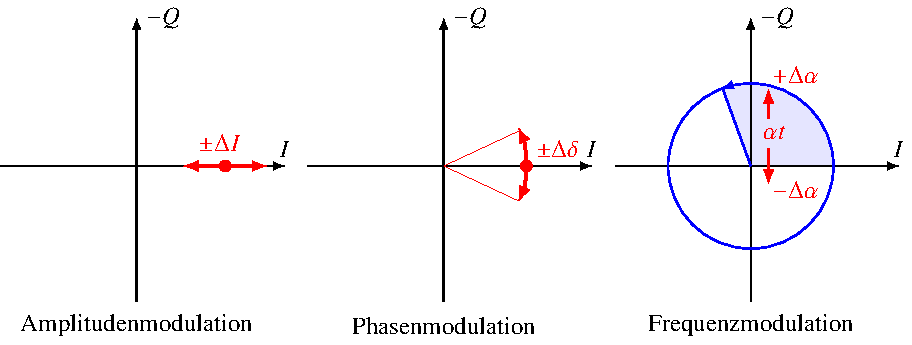
\includegraphics{applications/qam/images/amfmpm.pdf}
\caption{Amplitudenmodulation (links), Phasenmodulation (mitte) und
Frequenzmodulation in der $I$-$Q$-Ebene.
Frequenzmodulation ensteht durch eine Drehung in der $I$-$Q$-Ebene
mit der Kreisfrequenz der gewünschten Frequenzänderung.
\label{qam:figure:amfmpm}}
\end{figure}
Statt der Amplitude kann auch die Phase des Trägersignals moduliert werden.
Dazu muss $\omega t$ ersetzt werden durch $\omega t + \delta$.
Der konstante unmodulierte Vektor $\vec{v}_0$ in der $I$-$Q$-Ebene erzeugt
das modulierte Signal
\begin{align*}
D_{\omega t + \delta}
\vec{v}_0
&=
D_{\omega t}\underbrace{D_{\delta} \vec{v}_0}_{\displaystyle=\vec{v}(t)}.
\end{align*}
Eine Phasenänderung um den Winkel $\delta$ entsteht also dadurch, dass
man den Vektor $\vec{v}_0$ in der $I$-$Q$-Eben um $\delta$ dreht.
Dieses Modulationsverfahren heisst {\em Phasenmodulation}.
Abbildung~\ref{qam:figure:amfmpm} zeigt in der Mitte die Transformation
in der $I$-$Q$-Ebene, die Phasenmodulation bewirkt.

Mit reiner Amplitudenmodulation lässt sich kein Stereosignal übertragen.
Sind $L(t)$ und $R(t)$ die beiden Stereokanäle, dann erfolgt die
Amplitudenmodulation typischerweise mit $I(t)=1+L(t)+R(t)$,
wobei man wieder $L(t)+R(t)<1$ voraussetzen muss.
Ein reiner AM-Empfänger wird also nur das Audio-Signal $A(t)=L(t) + R(t)$
empfangen.

Um die Stereoinformation zu übermitteln, muss zusätzlich die Differenz
$L(t)-R(t)$ übermittelt werden.
Das C-QUAM Verfahren ({\bf C}ompatible {\bf Qu}adrature {\bf A}mplitude
{\bf M}odulation) verwendet dafür $Q(t)=L(t)-R(t)$.
Man darf annehmen, dass $L(t)-R(t)$ klein ist.
Dann befinden sich die Punkte $(I(t),Q(t))$ immer in der
Nähe der $I$-Achse, was sich in einer kleinen Verschiebung
\[
\delta = \arctan\frac{Q(t)}{I(t)} = \arctan\frac{L(t)-R(t)}{1+L(t)+R(t)}
\]
der Phase des übermittelten Signals äussert.
Der Betrag des Vektors $\vec{v}(t)$ ist dagegen
\begin{align*}
|\vec{v}(t)|
&=
\sqrt{
(1+L(t)+R(t))^2
+
(L(t)-R(t))^2
}
=
(1+L(t)+R(t))
\sqrt{
1+
\biggl(
\frac{L(t)-R(t)}{1+L(t)+R(t)}\biggr)^2
}
\\
&\simeq 1+L(t)+R(t),
\end{align*}
weil der zweite Summand unter der Wurzel klein ist.
Die $Q$-Komponente ändert also nicht wirklich etwas am Signal, welches
ein AM-Empfänger empfängt.

Um dem Emfpänger zu signalisieren, dass eine Stereoübertragung
vorliegt, wird $Q(t)$ zusätzlich ein Pilotton von 25\,Hz hinzugefügt.
Da nicht C-QUAM-taugliche Empfänger die Phasenschwankungen nicht erkennen
können, werden sie vom Pilotton auch nicht gestört.

\subsubsection{Frequenzmodulation}
Bei der {\em Frequenzmodulation} des UKW-Radios wird die Trägerfrequenz
im Takt des zu übertragenden Tonsignals verändert.
Lässt sich dies auch mit Hilfe der Signale $I(t)$ und $Q(t)$
beschreiben?
Welche Funktionen $I(t)$ und $Q(t)$ muss man wählen?

Ist das zu übertragende Audiosignal $0$, dann wird nur der unveränderte
Träger ausgestrahlt.
Dies lässt sich dadurch erreichen, dass man für $\vec{v}(t)$ den
konstanten Vektor $\vec{v}(t)=\vec{v}_0=(1,0)^t$ wählt.

Das ausgestrahlte Signal $s(t)$ entsteht als erste Komponente
des Vektors $D_{\omega t}\vec{v}(t)$.
Für konstantes $\vec{v}(t)=\vec{v}_0$ oszilliert es mit der Kreisfrequenz
$\omega$.
Will man, dass es schneller oszilliert, dann muss die Frequenz $\omega$
erhöht werden.
Möchte man die Frequenz um $\alpha$ steigern, dann muss man $\omega$
durch $\omega+\alpha$ ersetzen.
Das modulierte Signal ist dann
\[
\begin{pmatrix}
s(t)\\c(t)
\end{pmatrix}
=
D_{(\omega+\alpha)t} \vec{v}_0
=
D_{\omega t} \underbrace{D_{\alpha t} \vec{v}_0}_{\displaystyle=\vec{v}(t)}.
\]
Dies ist gleichbedeutend damit, dass man den Vektor $\vec{v}_0$ in der
$I$-$Q$-Ebene mit der Winkelgeschwindigkeit $\alpha$ dreht und so
$\vec{v}(t)$ erhält.
Daraus liest man ab, dass für die Signale $I(t)$ und $Q(t)$
\begin{equation}
\begin{pmatrix}I(t)\\Q(t)\end{pmatrix}
=
D_{\alpha t}\vec{v}_0
\qquad\Rightarrow\qquad
\left\{
\quad
\begin{aligned}
I(t)&=\cos\alpha t\\
Q(t)&=\sin\alpha t
\end{aligned}
\right.
\end{equation}
gilt.
Insbesondere kann man auch die Frequenzmodulation mit der
Quadratur-Amplituden-Modulation realisieren.
Abbildung~\ref{qam:figure:amfmpm} zeigt rechts symbolisch die
Kreisbewegung in der $I$-$Q$-Ebene, die Frequenzmodulation bewirkt.

\subsubsection{Analoges Farbfernsehen}
Die Entwicklung des analogen Farbfernsehens sah sich vor die Aufgabe 
gestellt, zusätzlich zur bereits im Schwarz-Weiss-Fernsehen übertragenen
Helligkeit (Luminanz, Y) die Farbinformation zu übermitteln.
Üblich ist dabei die Verwendung des YUV-Farbraumes, für den die zusätzlichen
Signale $U=R-Y$ und $V=B-Y$ benötigt werden, welche die Farbinformation
codieren.
Für ein farbloses Bild sind $U=0$ und $V=0$.

Das Problem ist also, zusätzlich zum Luminanzbild, welches bereits
amplitudenmoduliert übertragen wird, den Farbvektor $(U,V)^t$ zu
übertragen.
Es liegt daher nahe, dafür die Quadratur-Amplituden-Modulation zu
verwenden.
Im in Europa üblichen PAL-System wurde für den Träger für das Farbsignal
die Frequenz 4.43361875\,MHz verwendet.
Da ein Phasenfehler im Empfänger zu einer Drehung des Farbvektors
und damit zu einer auffälligen Verschiebung der Farben auf dem Farbkreis
führen würde, muss der Sender dem Empfänger die genaue Phase mitteilen.
Am Anfang jeder Zeile wird daher eine etwa zehn Perioden langer ``PAL-Burst''
übermittelt, den der Empfänger dazu verwenden kann, die Phase des
Farbträgers zu bestimmen.

Zusätzlich invertiert das PAL-System die Phase des Farbträgers
aufeinanderfolgender Zeilen, so dass sich Farbfehler durch Phasenfehler
auf aufeinanderfolgenden Zeilen wegmitteln.
Im PAL-System steht also Farbinformation jeweils nur für Paare von Zeilen
zur Verfügung und nur mit einer Dichte, die durch die Frequenz des Farbträgers
begrenzt ist.
Die effektive Farbauflösung eines PAL-Farbfernsehbildes ist daher halb so
gross wie die Helligkeitsauflösung.
Da auch die Farbauflösung des menschlichen Auges kleiner ist als die
Helligkeitsauflösung, ist diese Einschränkung des Systems von Auge nicht 
erkennbar.

\subsubsection{FSK und PSK}
Für die digitale Signalübertragung braucht man minimal die Fähigkeit,
zwei Zustände zu übermitteln, die man aber exakt wiedererkennnen können muss.
Frequency-Shift-Keying (FSK) ist ein Verfahren, welches zwei digitale Zustände
durch verschiedene Frequenzen codiert, es ist also ein
Frequenzmodulationsverfahren, von dem im vorangegangenen Abschnitt
bereits gezeigt wurde, wie es mit der Quadratur-Amplituden-Modulation
realisierbar ist.

Phase-Shift-Keying (PSK) verwendet stattdessen eine Phasenverschiebung
des Trägersignals.
Eine Phasenverschiebung um den Winkel $\varphi$ kann realisiert werden,
indem man eine Drehung um den Winkel $\varphi$ vorschaltet, also die
Drehmatrix $D_{\varphi}$ einfügt.
Besonders einfach ist eine Phasenverschiebung um den Winkel
$\varphi=180^\circ$, 
\[
D_{\varphi}
=
\begin{pmatrix}
\cos180^\circ&          - \sin180^\circ \\
\sin180^\circ& \phantom{-}\cos180^\circ
\end{pmatrix}
=
-E.
\]
Diese Phasenverschiebung wird also dadurch realisiert, dass man das
Vorzeichen von $I$ und $Q$ ändert.
Verwendet man den Vektor $(1,0)^t$ zur Codierung einer logischen
$\texttt{0}$, dann codiert der Vektor $(-1,0)^t$ eine logische $\texttt{1}$.
Auch PSK ist also mit Quadratur-Amplituden-Modulation realisierbar.

\subsubsection{Quantisierte QAM}
Mit Quadratur-Amplituden-Modulation lässt sich ein beliebiger Vektor
in der $I$-$Q$-Ebene übertragen.
Bei PSK wurden nur die Punkte $(1,0)$  und $(-1,0)$ in der $I$-$Q$-Ebene
verwendet.
Nach der Demodulation erhält man Vektoren, die wegen Fehlern nicht
exakt mit den ursprünglichen Vektoren übereinstimmen.
Da man aber nur die beiden logischen Zustände unterscheiden können muss,
kann man alle Vektoren mit $I>0$ als logische \texttt{0} decodieren
und Vektoren mit $I<0$ als logische \texttt{1}.

Statt nur zwei Zustände \texttt{0} und \texttt{1} zu codieren, könnte man
ein grössere Zahl von Punkten in der $I$-$Q$-Ebene verwenden, wie in
Abbildung~\ref{figure:qam:konstellation} dargestellt.
Die Punkte werden auch {\em Symbole} genannt.
Ein empfangener Vektor wird wegen Übertragungsfehlern nicht exakt mit
dem ursprünglichen Vektor übereinstimmen.
Zur Decodierung suchen wir dasjenige Symbol, welches dem Vektor am
nächsten liegt.
Man teilt also die Ebene in Teilgebiete $T_{\vec{v}_k}\subset \mathbb R^2$
zu jedem Symbol $\vec{v}_k$ auf.
Fällt der empfangene Vektor $\hat{v}$ in das Teilgebiet des Symbols
$\vec{v}_k$, also $\hat{v}\in T_{\vec{v}_k}$, dann decodieren wir ihn
als das Symbol $\vec{v}_k$.

\begin{figure}
\centering
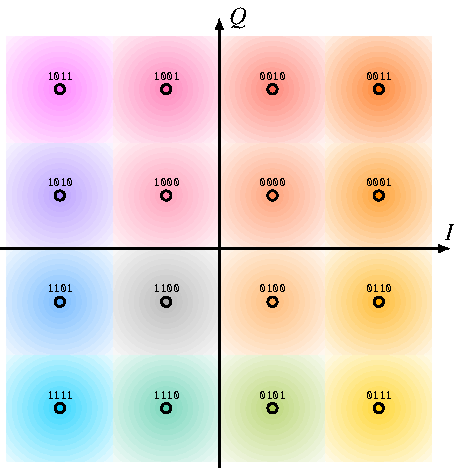
\includegraphics{applications/qam/images/konstellation.pdf}
\caption{Konstellationsdiagramm für quantisierte QAM mit 16 verschiedenen
Symbolen.
Mit jedem Symbol werden vier Bit codiert.
Zu jedem Symbol gehört ein quadratisches Gebiet gleicher Farbe.
Fällt der empfangene Vektor in eines dieser Gebiete, wird er als
das zugehörige Symbol decodiert.
\label{figure:qam:konstellation}}
\end{figure}

Im Beispiel der Abbildung~\ref{figure:qam:konstellation} können 16 
verschiedene Vektoren unterschieden werden, die man mit vierstelligen
Binärzahlen identifizieren kann.
Mit jedem Symbol werden also vier Bit übertragen.
Dieses Verfahren heisst auch 16-QAM und wird bei DVB-T verwendet.

Die Punkte-Menge $\vec{v}_k$ heisst auch die {\em Konstellation}
des Verfahrens.
Durch feinere Aufteilung können mehr Bits pro Symbol übertragen werden,
wie in Tabelle~\ref{table:qam:xqam} zusammengstellt.
Abbildung~\ref{figure:qam:analyzer} zeigt, wie sich die Messung eines 256-QAM 
Signals auf einem Vector Signal Analyzer darstellt.

Für ungerade Potenzen von $2$ kann das Konstellationsdiagramm kein
Quadrat sein.
Für $k$ ungerade kann man aber $2^k$ Punkte erhalten, indem man
dem Quadrat der $2^{k-1}$ Punkte der Konstellation von $2^{k-1}$-QAM
vier Rechtecke mit jeweils $2^{k-1}/4=2^{k-3}$ Punkten hinzugefügt, daraus
ergibt sich eine Konstellation mit
$2^{k-1}+4\cdot 2^{k-3}=2^{k-1}+2^{k-1}=2^k$
Punkten (Abbildung~\ref{qam:figure:qam-konstellation} Mitte).
In diesem hat das Konstellationsdiagramm also die Form
eines Kreuzes mit breite $2^{(k-1)/2}$ und Armlänge
$\frac32\cdot 2^{(k-1)/2}$.
Diese Konstellation wird manchmal auch Cross-QAM genannt.

\begin{table}
\centering
\begin{tabular}{rrcrl}
\hline
Bits&Symbole&Konstellation&Name&Anwendung\\
\hline
   2&      4&$  2\times   2$      &    4-QAM&DVB-S       \\
   4&     16&$  4\times   4$      &   16-QAM&V.29, DVB-T \\
   6&     64&$  8\times   8$      &   64-QAM&DVB-C, DVB-T\\
   8&    256&$ 16\times  16$      &  256-QAM&DVB-C       \\
  10&   1024&$ 32\times  32$      & 1024-QAM&            \\
  12&   4096&$ 64\times  64$      & 4096-QAM&DVB-C2, G.hn\\
  15&  32768&$128\times 256$ Kreuz&32767-QAM&ADSL        \\
\hline
\end{tabular}
\caption{Verschiedene Konstellationen für quantisierte QAM mit Anwendungen.
\label{table:qam:xqam}}
\end{table}

\begin{figure}
\centering
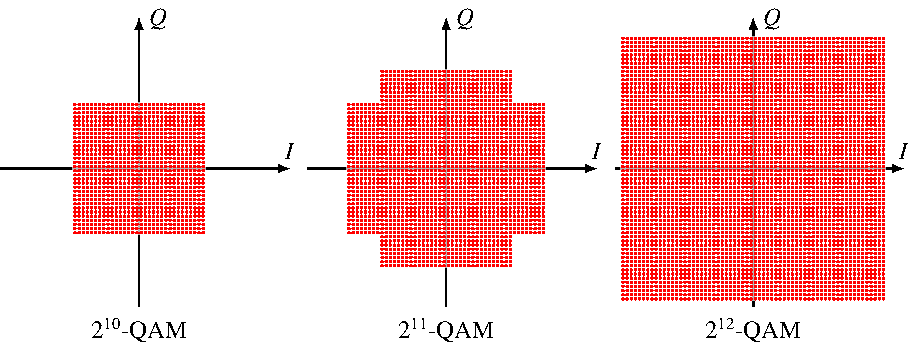
\includegraphics{applications/qam/images/qam.pdf}
\caption{Konstellationsdiagramme für $2^k$-QAM für verschiedene Werte von $k$.
\label{qam:figure:qam-konstellation}}
\end{figure}

\begin{figure}
\centering
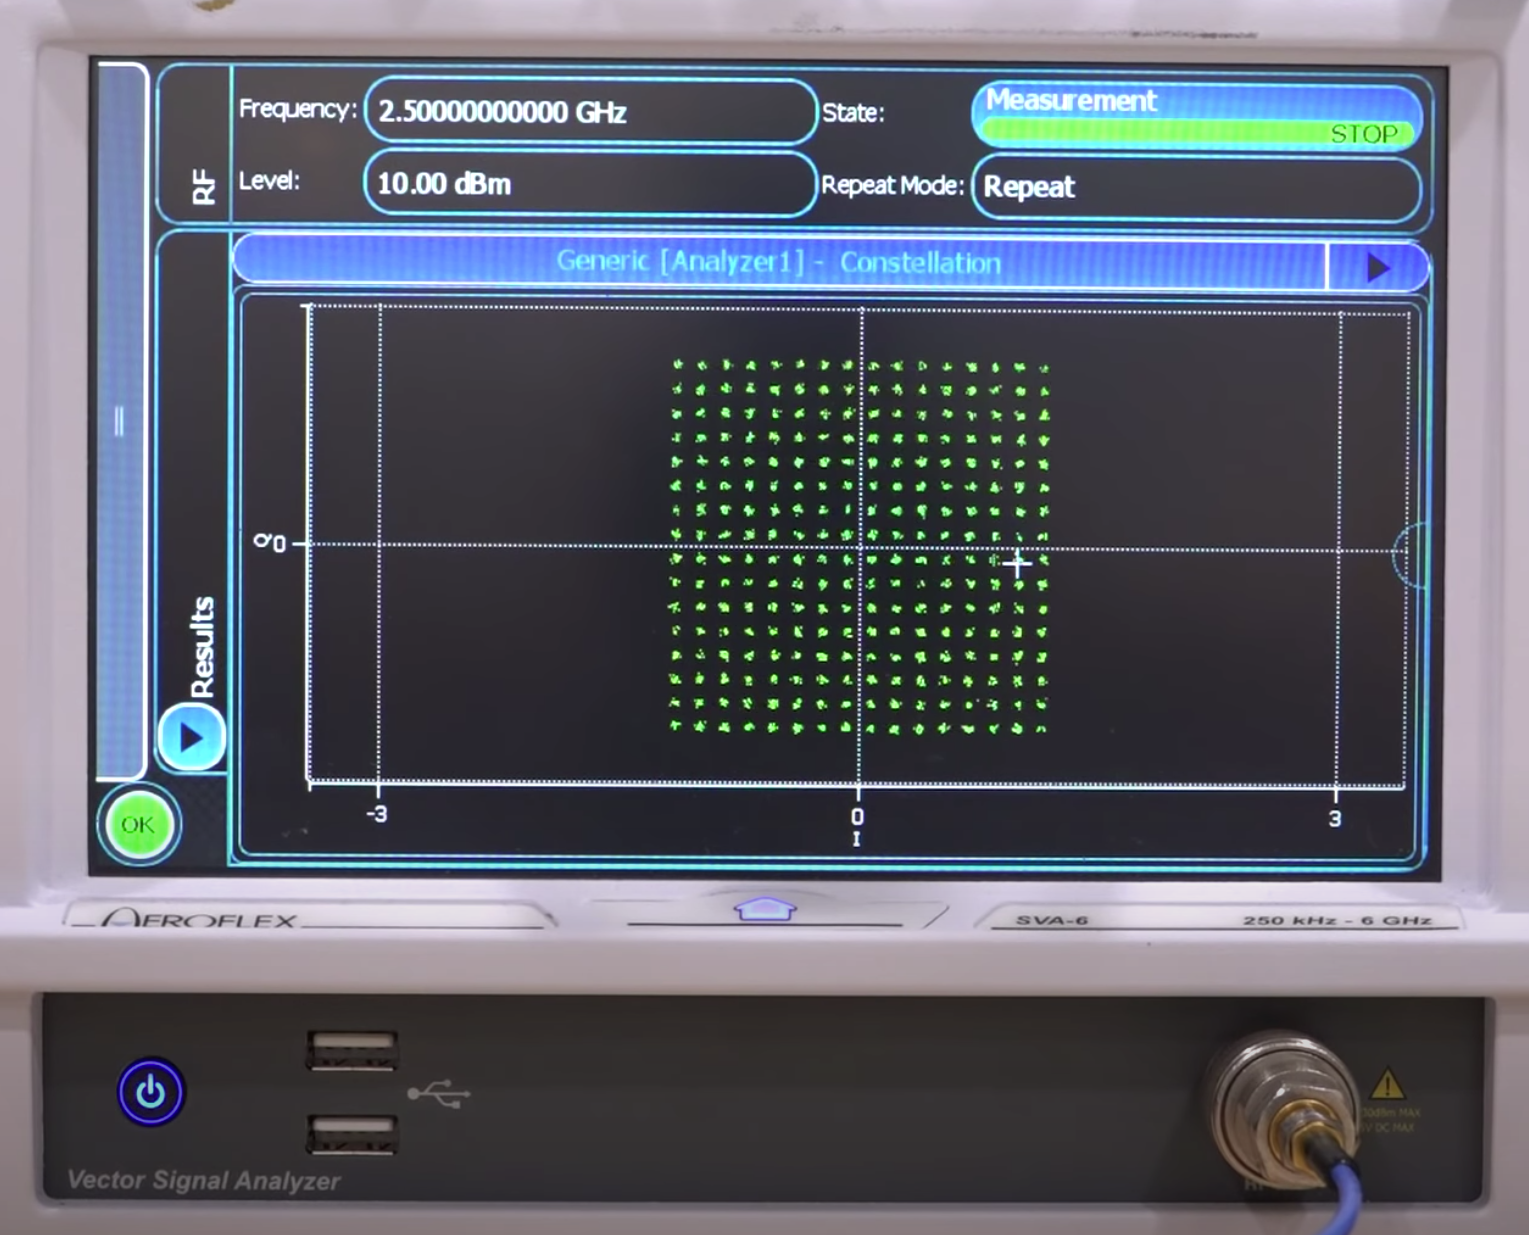
\includegraphics[width=1.0\hsize]{applications/qam/images/analyzer.png}
\caption{Messung des Konstellationsdiagramms eines 256-QAM Signals
mit einem Vector Signal Analyzer.
Man beachte die Beschriftung der Achsen mit \texttt{I} und \texttt{Q}.
(Ausschnitt aus dem Video \url{https://www.youtube.com/watch?v=uV3O3tpjmS8}
bei 26:36).
\label{figure:qam:analyzer}}
\end{figure}

\subsubsection{$n$-PSK}
Analog zum Vorgehen bei der quantisierten QAM kann auch PSK diskretisiert
werden.
Als Konstellationsdiagramm für $n$-PSK dienen $n$ Punkte auf einem Kreis,
die durch einen Winkel $2\pi/n$ getrennt sind.
In Abbildung~\ref{figure:qam:psk} ist das Konstellationsdiagramm für
$8$-PSK dargestellt.
\begin{figure}
\centering
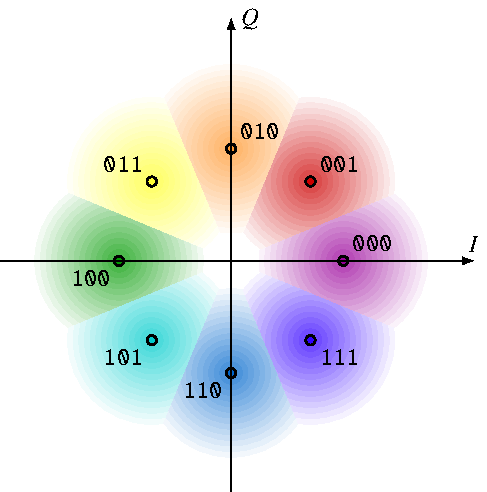
\includegraphics{applications/qam/images/psk.pdf}
\caption{Konstellationsdiagramm für 8-PSK 
\label{figure:qam:psk}}
\end{figure}

\subsubsection{Software Defined Radio}
Die vorangegangenen Beispiele haben illustriert, dass die
Quadratur-Amplituden-Modulation jedes besprochene Modulationsverfahren
realisieren kann.
Es ist nur nötig, einen Sender zu bauen, der Inputs $I(t)$ und $Q(t)$
entgegennimmt, die Modulation mit der Matrix $D_{\omega t}$ vornimmt
und das resultierende Signal $s(t)$ aussendet.
Auf der Empfängerseite braucht man eine physikalische Realisierung
der Matrix $D_{\omega_r t}$ und des Tiefpasses, der die demodulierten
Signal $\hat{I}(t)$ und $\hat{Q}(t)$ ausgibt.
Die Decodierung zum Beispiel als amplitudenmoduliertes Sprachsignal,
als frequenzmoduliertes Musiksignal oder als digitales 16-QAM-Signal
kann danach ausschliesslich in Software erfolgen.
Die Modulationsart eines solchen sogenannten {\em Software Defined Radio (SDR)}
wird also durch die Software definiert, welche die Signale $I(t)$ und $Q(t)$
erzeugt bzw.~die Signale $\hat{I}(t)$ und $\hat{Q}(t)$ analysiert.
SDR ermöglicht dem interessierten Hacker auch exotische Experimente,
wie das in Abbildung~\ref{qam:figure:digital} dargestellte fiktive
digitale Modulationsverfahren.

\begin{figure}
\centering
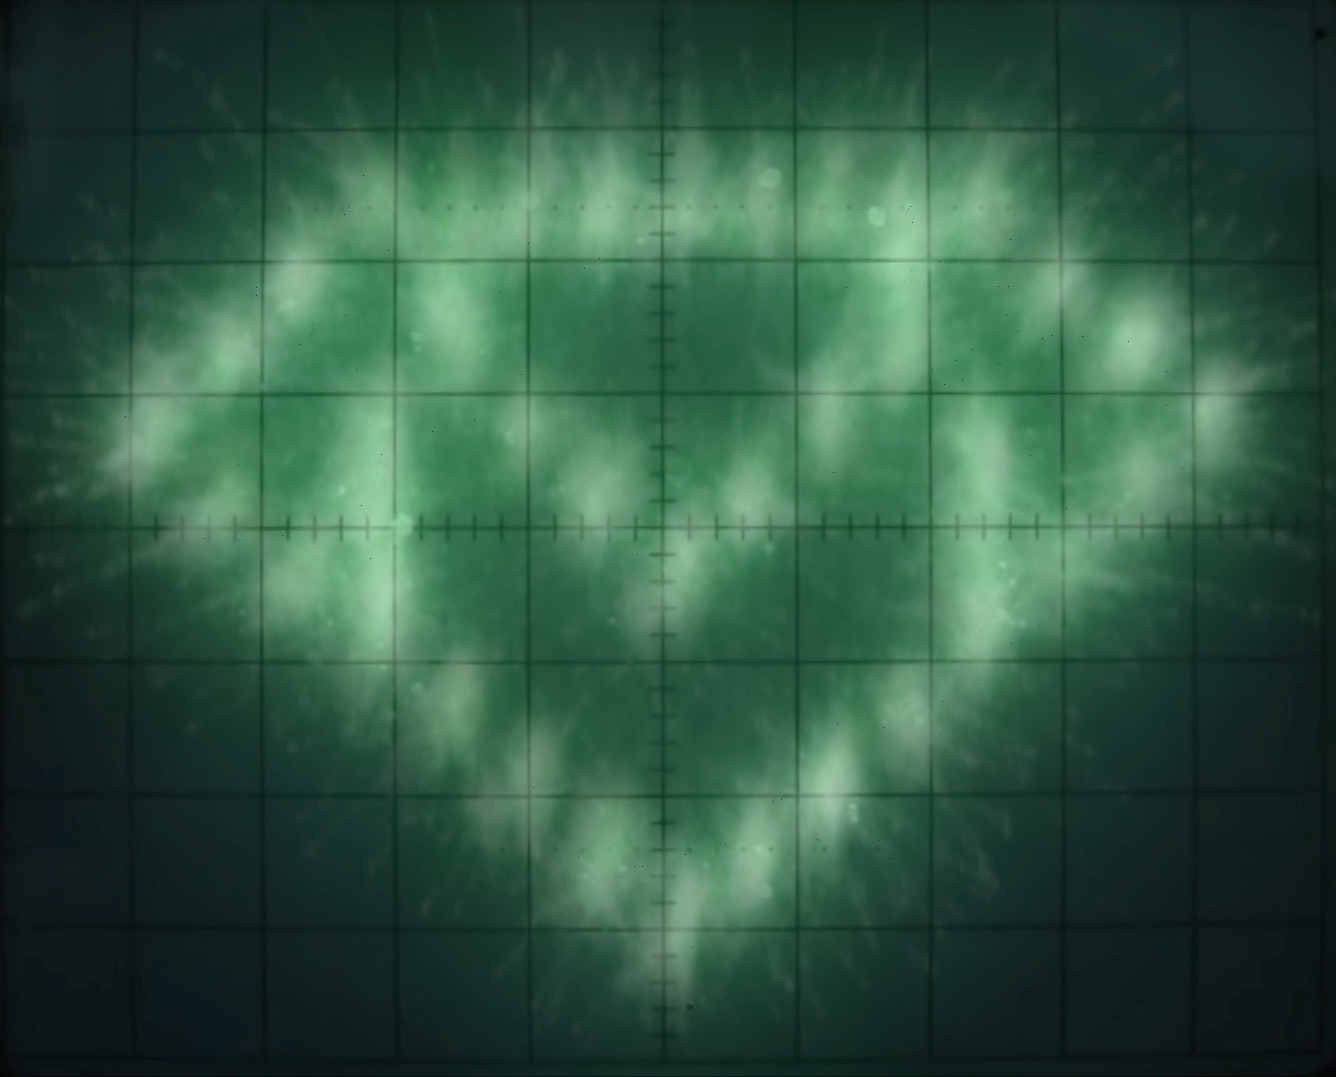
\includegraphics[width=0.7\hsize]{applications/qam/images/digital.jpg}
\caption{Konstellationsdiagramm für ein fiktives digitales
Modulationsverfahren, welches nur Punkte eines MathMan-Logos als
Symbole verwendet.
\label{qam:figure:digital}}
\end{figure}


